\section{Method} \label{sec:method}
The optimization of power regulation while minimizing loads, requires a model that can describe the power output and the loads of a wind farm. This section describes how this in implemented \newline
An overview of the optimization procedure used is illustrated in Figure \ref{fig:optim}.
The power output of a wind farm as well as the wake propagation in this wind farm are calculated using the FLORIS model \cite{FLORIS} (Section \ref{sec:floris}). Given a certain inflow profile the program FAST calculates the out of plane bending moments on a turbine. With the program MLife these bending moments are converted to a Damage Equivalent Load (DEL), which is a measure for the lifespan of a wind turbine \cite{MLife}. Both FAST and MLife are covered in Section \ref{sec:fast}. These DELs are pre-calculated for different situations, which are specified by four parameters, and stored in a look-up-table (LUT) so it can be quickly retrieved during optimization (Section \ref{sec:lut}). The optimization algorithm uses a cost function that combines the DEL and power data to find the optimal wind turbine configuration that has minimal loads while tracking a predefined reference power (Section \ref{sec:optimization}).

\begin{figure}
	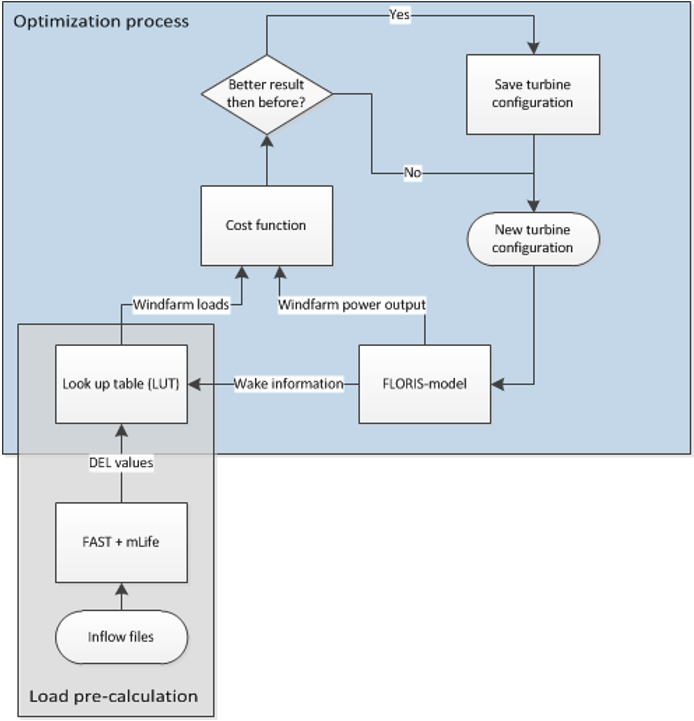
\includegraphics[width=\linewidth]{./Figures/OptimizationProcess.png}
	\caption{Overview of the optimization procedure.}
	\label{fig:optim}
\end{figure}


%\noindent

\subsection{FLORIS} The FLOw Redirection and Induction in Steady state (FLORIS) model is used to simulate the wind flow in a wind farm while also generating power output data. The model works as a function of the yaw misalignment and the axial induction\cite{Gebraad2016}. FLORIS is a parametric model fitted to high-fidelity data from a computational fluid dynamics simulation, making it a relative accurate model with low computation time\cite{Dijk2016}. 

\subsubsection{Wake modelling}
\label{wakemodel}
%As can be seen in Figure \ref{fig:wake}, 
FLORIS generates a wake model which divides the wake into three different zones as shown in Figure \ref{fig:wake}. These zones are defined as the near wake, the far wake, and the mixing zone, and are denoted by $q$. Each zone has its own function for the zone diameter and wind speed, which are calculated by FLORIS using Equations (\ref{eq:Dw} to \ref{eq:c}). 


\begin{figure}
  	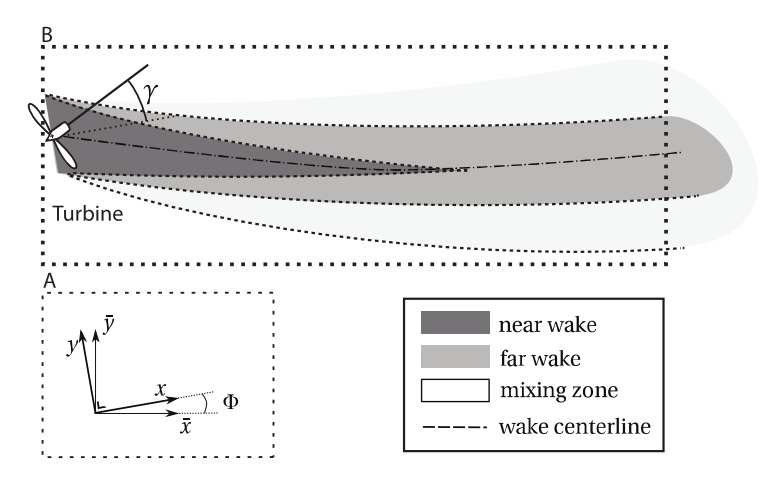
\includegraphics[width=\linewidth]{./Figures/WakeFLORIS.png}
  	\caption{Simplified top view representation of a wake of a turbine by FLORIS.\cite{Gebraad2016}   }
	\label{fig:wake}
\end{figure}

The diameter sizes of the wake zones are calculated using Equation \ref{eq:Dw}. Let the $D_i$ denote the rotor diameter of the $i${\textsuperscript{th}} turbine, $k_e$ a coefficient that describes expansion of the zones, and $m_{e,q}$, the expansion factor as used by Gebraad \cite{Gebraad2016}. The diameter size of third wake zone $D_{w,q,i=3}$ is frequently used further in the paper. for that reason, unless specified otherwise, is this what is meant when referred to a wake diameter. Also is the simplified notation $D_w$ is used for easer reeding. This diameter $D_w$ increases proportionally with the longitudinal distance, downwind distance $x$, away from the wake-generating turbine. (For orientation see Figure \ref{fig:optim}.)
\begin{equation}
\label{eq:Dw}
D_{w,i,q}(x) = max({D_i + 2k_em_{e,q}([x - X_i],0} )
\end{equation}
The velocity in the wake can also be related to this downwind distance $x$. As shown in Equation \ref{eq:Uw}, is the wake velocity an argument of the wake decay coefficient $c_{i,q}(x)$ and the axial induction factor $a_i$. This axial induction factor is a measure for the wind speed reduction behind a turbine relative to its own rotor speed. (<--note bart). The wake decay coefficient describes the decay of velocity for each wake zone and is defined in Equation \ref{eq:c}. In this equation is the model parameter $M_{U,q}$ a ...depended of the wake zones and yaw angle\cite{Gebraad2016}. And the $X_i$ is ... ?

\begin{equation}
\label{eq:Uw}
U_{w,i}(x,y) = U_i\left( {1-2a_{i}c_{i,q}(x)} \right)
\end{equation} 

\begin{equation}
\label{eq:c}
c_{i,q}(x) = \left[ \frac{D_i}{D_i + 2k_em_{U,q}(\gamma_i)[x - X_i]} \right]^2
\end{equation}



%//programming tool for the simulation of dynamic (load) responses of wind turbines (by NREL) 
%\noindent
%(klopt deze cite nog met deze benaming?),-->
\subsection{FAST \& MLife} FAST is a dynamic turbine model\cite{Jonkman2005}. Among others, it computes the out of plane bending moments of the turbine blades, which are explained earlier in the method section. Since these out of plane bending moments fail to give direct information about the effect on the lifetime of a turbine, the program MLife is used to convert the bending moment to damage equivalent loads (DELs). These DELs are... \cite{Mlife}.


\begin{figure}
  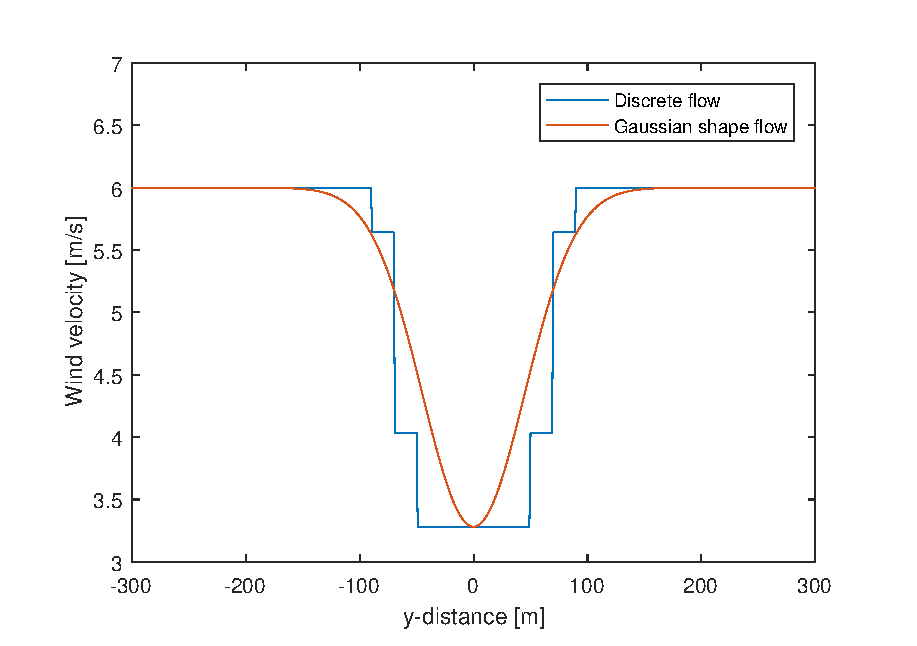
\includegraphics[width=\linewidth]{./Figures/PlotGausDiscWakeDWake180U6yaw0.eps} %Plot with Gauss vs Discr flow, Dwake = 180, u_mean = 6, yaw = 0
  \caption{Discrete wake versus Gaussian wake} %for Dwake = 180 m, U = 6 m/s, and yaw = 0
  \label{fig:disgaus}
\end{figure}

%\noindent

\subsubsection{Flow field}
FAST uses external input files for its simulations. One of these input files contains the flow field information. It contains the data of the wind flow as it falls on the turbine blades. This study made this wind data more representative for real life by implementing both a more realistic wake distribution, the Gaussian distribution, as well as natural phenomena, the shear effect.

\paragraph{Gaussian wake}
FLORIS describes a discrete flow field of a wake, with three zones. The flow field of the wake in FLORIS is calculated with equations (\ref{eq:Dw} to \ref{eq:c}). The wake is divided into three zones as described in section \ref{wakemodel}. A real wake, however, does not have these discrete zones. To create a more fluent transition between the different wake-zones, a Gaussian distribution of the flow field is introduced\cite{Bastankhah2016}. The wake shape difference can be seen in Figure \ref{fig:disgaus}.  The Gaussian distribution is calculated as follows: 

\begin{equation}
\label{eq:gaus}
G(y, z) = A [e^{-(\frac{y^2}{2\sigma_y} + \frac{z^2}{2\sigma_z})}]
\end{equation}
The amplitude of the Gaussian, $A$, is set to be equal to the velocity loss of the inner wake zone, $U_{w,1}$, as generated by FLORIS. $\sigma_y$ and $\sigma_z$ reflect the Gaussian standard deviation in horizontal and vertical direction, respectively. These standard deviations are related wake diameter $D_{w}$ following Equation \ref{eq:sigm},
\begin{equation}
\label{eq:sigm}
\sigma_y,\sigma_z = \frac{D_{w}}{n} 
\end{equation}
\\
Where fit parameter $n$ can be modified to change the width of the Gaussian. Consequently, making it possible to fit a Gaussian to the wake zones of FLORIS (Figure \ref{fig:disgaus}). Future versions of FLORIS will also have this Gaussian distribution implemented. (clearly note the importance of the relation between the Gaussian and the wakes from FLORIS!!) 

\paragraph{Wind shear} \label{sec:windshear}
An other aspect added to improve the accuracy of the wind data is wind shear. This natural phenomenon is the result of earths surface slowing the wind down closer to the ground. This results in a significant difference in wind speed over the height ranges of the turbine, which has a significant effect on the DELs\cite{Firtin2011}.  The velocity distribution is calculated as follows: 
\begin{equation}
\label{eq:shear}
v = v_{ref} \left[\frac{h}{h_{ref}}\right]^\alpha
\end{equation}
(bron voor deze Eq?)
where $v$ and $v_{ref}$ are the velocity at heights $h$, and $h_{ref}$  respectively. Value $\alpha$ is the wind shear coefficient which depends on different factors. The coefficient $\alpha$  reflects terrain type, and is for this paper fixed at value 0.1 representing a surface close to ocean and smooth ground \cite{Firtin2011}. Figure \ref{fig:windshear} shows the flow fields of a wake for both before and after the implementation of shear, clearly showing the effect of the shear effect.

\begin{figure}
	\centering
	\begin{subfigure}[b]{0.50\textwidth}
		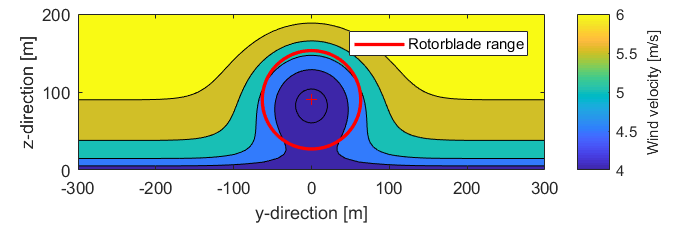
\includegraphics[width=\linewidth]{./Figures/PlotwithshearU6D220.png} %Plot with windshear u_mean = 6
		\caption{Flow field with wind shear.}
		\label{fig:windsh}
	\end{subfigure}
	
	\begin{subfigure}[b]{0.50\textwidth}
		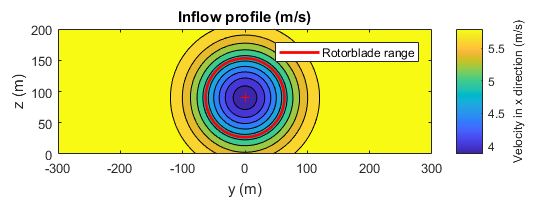
\includegraphics[width=\linewidth]{./Figures/PlotwithoutshearU6D220.png} %Plot without windshear u_mean = 6
		\caption{Flow field without wind shear}
		\label{fig:nowindsh}
	\end{subfigure}
	
	\caption[Two Gaussian flow fields]{Gaussian wind fields with a free stream velocity of 6 $m/s$ at a height of 90 $m$. The outer diameter of de wake is 220 $m$ and the diameter of the rotor blades is 126.4 $m$.}
	\label{fig:windshear}
\end{figure}




\begin{table}[h]
	%\renewcommand{\arraystretch}{1.3} 
	\caption{Overview of the minimum value, maximum value, and step size of the parameters, diameter of outer wake zone (Dwake), free stream wind speed (U), yaw of the turbine (yaw), and the center to center distance between the center of the turbine and the center of the wake (y wake).}
	\centering
	\label{tab:pars}
	\begin{tabular}{lccc}
		\hline
	 	& Minimum & Maximum & Step-size \\ 
		\hline
		Dwake & 180 & 330 & 25 \\
		U & 6 & 8 & 2 \\
		yaw & -30 & 30 & $^*$ \\
		y wake & -250 & 250 & 10 \\
		\hline
	\end{tabular}
$^*$Input values for yaw are [-30, -10, -5, 0, 5, 10, 30].
\end{table}

%\noindent
\subsection{LUT} \label{sec:lut}
 To reduce computational time during optimization a look-up table (LUT) is created. The LUT is created using FAST and MLife, and it contains a a large number of DEL values for a wide variety of wind field conditions on a wind turbine.
These different conditions are described by the ranges of the parameters, which can be seen in Table \ref{tab:pars}. The parameters are wake characteristics which can be extracted from FLORIS. The parameters chosen for the LUT are:\begin{itemize}
	\item the free stream wind speed, U
	\item the outer diameter of the wake, Dwake
	\item the yaw of the turbine, yaw  
	\item the center to center distance between the turbine and the wake, y wake 
\end{itemize}   
 To save calculation time, the LUT parameters are discretized, given each parameter a certain step-size. This step-size is chosen such that interpolation will give a representative result. For each parameters step-sizes are selected, as shown in Table \ref{tab:pars}. With the use of the pre-calculated LUT, online optimization can be realized.



 This paper uses the wake diameter as a parameter to characterise the wakes. However, as stated before are the diameter of the wake, the downwind distance and the windspeed reduction behind the turbine(Udef) related by fitting equations. This means that the distance and the Udef could have been used as parameter just as well. The choice for the diameter comes since Floris searches for the best fit of the shape of a wake in the LUT data. And the diameter gives a more direct interpretation of the shape of the wake than the others do, subsequently meaning that the diameter comes more intuitively.

 
 

%\noindent
\subsection{Optimization} \label{sec:optimization}
For the optimization, a trade off has to be made between power regulation and load minimization. This trade off can be defined by a cost function \cite{Marden2013}\cite{Dijk2016}. The optimal turbine configuration, defined by the yaw ad axial induction settings for all individual turbines, is found by minimization of this cost function. The optimization method used is game-theoretic approach\cite{Marden2013}. It preforms the simulation with different settings, searching for the best outcome. As further explained in section \ref{sec:gametheory}. 
 

\subsubsection{Cost Function} \label{sec:costfunction}

The cost function is a mixed-objective cost function, minimizing the combined loads without straying to far away from the reference power of the wind farm. It uses the power and load data from the simulations combined with optimization parameters $c$ and $P_bw$ to evaluate each turbine configuration case, defined as follows: 

\begin{equation}
\begin{aligned}
J(P,DEL) = c((P_{ref}-P(a_i,\gamma_i))/P_{bw})^2  + \\
(1-c)DEL(a_i,\gamma_i)/DEL_{base}
\end{aligned}
 \label{eq:costf}
\end{equation}
Where $c$ is the tuning parameter defining the relative importance of the power and loads optimization objectives. $P_{ref}$ is the desired power output of the wind farm that the regulation wishes to obtain. $P_{bw}$ and $DEL_{base}$ are the power and loads baselines respectively, to create normalized variables.
\newline

To obtain power production close to the reference, the power part of the cost function is a quadratic difference. As a result power outputs further away from the reference are heavily penalized. $P_{bw}$ is used to regulate at which power error the emphasis shifts to the loads.

\subsubsection{Game Theory} \label{sec:gametheory}
The game-theoretic approach uses random perturbations on the yaw angles and the axial induction factors to minimize the cost function. When new values for yaw and axial induction settings give an improvement regarding the cost function, the settings are saved and the process will be repeated with the new settings. Because of the fact it uses random perturbations, the game theoretic approach is an adequate optimizer to find the global minimum of the cost function.\cite{Dijk2016}




